% ---------------------------------------------------------------------------
% Anonymised manuscript for double-blind review.
% Do not add author names, affiliations, acknowledgements or funding statements
% to this file; the CFP requires the manuscript itself to carry none of them.
% Identifying information belongs in the separate cover letter.
% ---------------------------------------------------------------------------
\documentclass[11pt,a4paper]{article}

\usepackage[utf8]{inputenc}
\usepackage[T1]{fontenc}
\usepackage[english]{babel}
\usepackage{lmodern}
\usepackage[margin=1in]{geometry}
\usepackage{booktabs}
\usepackage{graphicx}
% Finds the figure whether it sits beside paper.tex (as on Overleaf) or in the
% repository's data/results/ directory.
\graphicspath{{./}{figures/}{data/results/}}
\usepackage{amsmath}
\usepackage{siunitx}
\usepackage[hidelinks]{hyperref}
\usepackage{apacite}          % APA-style citations, per the CFP
\usepackage{setspace}
\onehalfspacing

\sisetup{detect-weight=true, detect-family=true}
% FLOP/s is not an SI unit, so siunitx does not define it. Declaring it here
% keeps the throughput figures typeset consistently with the others.
\DeclareSIUnit{\flop}{FLOP}

% ICRR requires a title under 20 words that states what the paper does, with no
% question form and no subtitle. The previous title was a question with a
% subtitle and broke both rules.
\title{\textbf{Low-Cost Inference-Time Signals Outperform NLI Models and LLM
Judges at Detecting Unsupported Retrieval-Augmented Generation Answers}}
\date{}
\author{}

\begin{document}
\maketitle
\thispagestyle{empty}

\begin{center}
\begin{tabular}{@{}ll@{}}
\textbf{Section} & Natural Sciences \\
\textbf{Article type} & Original research \\
\textbf{Running head} & Low-cost signals for RAG hallucination detection \\
\textbf{Abstract word count} & 232 \\
\textbf{Manuscript word count} & 5,650 (excluding references and appendices) \\
\end{tabular}
\end{center}

\vspace{1em}

% ===========================================================================
\begin{abstract}
\noindent
Retrieval-augmented generation (RAG) is widely adopted to ground large language
models in external documents, yet RAG systems still produce fluent claims that
the retrieved context does not support. Most detection methods answer this with
a second, larger judge model, which is impractical for teams without that
budget. We ask how far one can get using only signals already available at
inference time on modest hardware. Over 150 question--context pairs built from
50 arXiv abstracts, generated with a 4-bit Qwen2.5-7B on a single 6\,GB consumer
GPU, we compare three such signals (token log-probability, self-consistency
across sampled generations, and NLI entailment against the retrieved
context) against a near-free lexical baseline and a 7B LLM-as-judge. Ground
truth is a two-annotator consensus ($\kappa = 0.78$). The ordering we found
inverts the one the literature assumes. Mean token log-probability, which costs
nothing beyond the generation itself, leads on AUROC at $0.849$ and is
statistically indistinguishable from a lexical baseline costing
\SI{41}{\milli\second}, while the NLI cross-encoder reaches only $0.669$ at
\SI{2.6}{\second} per query and the LLM judge attains a lower $F_1$ than the free
signal at \SI{5.0}{\second}. A stratified analysis shows the log-probability
result is not reducible to answer length. We also find the judge systematically
violates an explicit instruction in its own rubric, and that our strongest
manipulation elicits appropriate abstention more often than fabrication. For
resource-constrained deployments, the practical recommendation is to exhaust
free signals before paying for expensive ones.
\end{abstract}

\vspace{0.5em}
% ICRR: four to six keywords, and none that already appear in the title.
\noindent\textbf{Keywords:} token log-probability; self-consistency; factual
consistency; uncertainty estimation; annotation reliability; low-resource
evaluation

\vspace{1em}

% ===========================================================================
\section{Introduction}

Retrieval-augmented generation has become the default way to ground a language
model in knowledge it does not hold in its parameters
\cite{lewis2020retrieval}. Retrieving a relevant document and placing it in the
prompt is cheap, requires no fine-tuning, and lets a system answer questions
about material that postdates training. It does not, however, guarantee that the
model uses what it was given. RAG systems still emit confident, well-formed
statements that the retrieved passage does not support, and this remains one of
the most frequently cited obstacles to deploying them.

The dominant response is to check the output with a second model. An LLM judge,
prompted with the context and the answer, is asked whether the latter follows
from the former. This works, but it doubles inference cost and presumes access
to a model large enough to be trusted as an arbiter, an assumption that fails
precisely for the teams most exposed to the problem. A student group, a small
company, or anyone running on a single consumer GPU cannot casually add a
frontier-model call to every query.

That constraint motivates a narrower question. Rather than asking what the best
possible detector is, we ask how much can be recovered from signals that are
\emph{already present} when a model generates an answer, or that can be computed
by a model small enough to sit alongside the generator on the same card. Three
such signals appear in the literature. Token log-probability is free: the
generator computes it whether or not anyone reads it. Self-consistency requires
re-sampling the same prompt and measuring agreement across the samples
\cite{manakul2023selfcheckgpt}. NLI entailment scores the answer against its
context using a pretrained cross-encoder of a few hundred million parameters
\cite{laban2022summac}.

These have generally been studied in isolation, or benchmarked against judge
models that assume the very budget the approach is meant to avoid. We compare
all three head to head under identical retrieval and generation conditions, on
hardware chosen to be representative of a constrained deployment, and we treat
cost as a first-class outcome rather than a footnote. If a signal is ten times
better but a thousand times more expensive, that is a different recommendation
from the one an accuracy table alone would give.

Our contributions are the following. We report a controlled comparison of three
inference-time detection signals, measured against both a near-free lexical
baseline and an LLM-as-judge reference point, with per-signal latency measured
under identical conditions. We evaluate under three retrieval conditions of
decreasing quality, which shows the signals failing in different places rather
than merely ranking against one another. And we report a result that runs
against the expected ordering: on our data the cheapest signal is the most
accurate, and the two most expensive are among the least.

We state the research question directly. \emph{Among detection signals available
at inference time on a single consumer GPU, how does detection accuracy relate to
computational cost, and is any signal's advantage large enough to justify its
expense?} Our hypothesis on entering the study was that NLI entailment would
lead, followed by self-consistency, with log-probability a distant third. The
data reversed that ordering.

% ===========================================================================
\section{Background and literature}

\paragraph{Self-consistency.}
SelfCheckGPT \cite{manakul2023selfcheckgpt} introduced a family of zero-resource,
black-box hallucination detectors that sample a model repeatedly and measure
agreement across the samples. The intuition is that a model with genuine
knowledge of a fact will reproduce it across stochastic decodes, whereas
fabricated content will vary. Several scoring variants were proposed, of which
the NLI-based one offered the best accuracy-to-cost balance. The method requires
no access to model internals, which is its main appeal, but it multiplies
inference cost by the number of samples.

\paragraph{NLI-based factual consistency.}
A second line of work treats the problem as natural language inference: a
generated claim is checked for entailment against its source. Applying
sentence-level NLI models to document-level inputs is not straightforward, since
the granularity of the training data and the task differ. SummaC
\cite{laban2022summac} addressed this by segmenting documents into sentences,
computing pairwise entailment, and aggregating the resulting matrix, which
recovered much of the performance earlier work had failed to obtain. FActScore
\cite{min2023factscore} pushed the decomposition further, breaking generations
into atomic facts and scoring each independently, a distinction that becomes
relevant to our results in Section~\ref{sec:results}.

\paragraph{Probability-based signals.}
Token-level output probabilities have been explored as a low-cost proxy for
model uncertainty, on the intuition that a model is less confident when
generating content it cannot ground. This is the cheapest signal available,
requiring no additional inference. It is also the most frequently dismissed:
language models are known to be confidently wrong, and mean token probability
is confounded with output length and with generic phrasing.

\paragraph{Gap.}
Prior work largely evaluates these signals separately, or against large judge
baselines. We are not aware of a direct comparison of all three under a shared,
explicitly resource-constrained setup with cost measured alongside accuracy,
which is the gap this study addresses.

% ===========================================================================
\section{Methods}

\subsection{Design}

This is a quantitative benchmarking study with a within-items design: every
detection signal is computed on the same 150 generated answers, so signals are
compared on identical material rather than across separate samples. Retrieval
quality is manipulated in three levels (Section~\ref{sec:conditions}) to test
whether signal behaviour depends on how the retrieval failed, and the outcome
measure is agreement with a human consensus label. The design suits the question
because the comparison of interest is relative, not absolute: we need to know
which signal separates supported from unsupported answers best on a fixed budget,
which requires holding the generator, the corpus, the prompt and the hardware
constant while varying only the detector.


\subsection{Data, materials, and sources}

The task is closed-domain question answering over scientific abstracts, with
verification against the retrieved passage. We chose abstracts because their
claims are narrow, factual and largely unambiguous to check, which matters when
the ground truth must be produced by hand.

The corpus is 50 arXiv abstracts (median 1{,}235 characters, published
2022--2026), assembled from six related queries within one area: hallucination
in RAG, faithfulness and groundedness, RAG evaluation benchmarks, factual
consistency, attribution and citation, and uncertainty estimation. All are
restricted to \texttt{cs.CL} so that abstract length and structure stay
comparable. Results from the six queries were merged round-robin so that no
single query dominates.

Drawing from several related queries rather than one is deliberate. A corpus
built from a single narrow query yields fifty near-interchangeable abstracts, in
which every distractor is an equally hard negative and the retriever cannot
discriminate between them. Six related-but-distinct facets give a range of
distractor difficulty, which Section~\ref{sec:conditions} uses as a controlled
variable. Survey papers and abstracts shorter than 700 characters were excluded
during construction, since neither supports the question templates below.

\subsection{Procedure and analysis}

\subsubsection{RAG pipeline}

Retrieval is embedding-based, using \texttt{all-MiniLM-L6-v2}
\cite{reimers2019sentencebert} with cosine similarity over L2-normalised
vectors. Each abstract is embedded once as title plus abstract.

The generator is Qwen2.5-7B-Instruct, 4-bit quantised (Q4\_K\_M, approximately
\SI{4.7}{\giga\byte}), served locally through Ollama. Ollama was chosen over
alternatives for one decisive reason: it exposes per-token log-probabilities
through its API, and the first signal under study \emph{is} token
log-probability. Its ability to evict a model from VRAM on demand is also what
makes the one-model-at-a-time discipline of Section~\ref{sec:setup} practical.

We considered adding a hosted API model as a second generator and rejected it.
Generation requires 900 calls (150 pairs $\times$ six samples each), which
exceeds the free-tier daily quotas available to us, and free-tier support for
log-probabilities is inconsistent across providers. Routing generation through a
hosted API would also sit awkwardly with a paper arguing for cheap, local,
reproducible detection. Every model reported in this paper, including the judge
baseline of Section~\ref{sec:eval}, therefore runs locally on the hardware
described in Section~\ref{sec:setup}.

Three fixed question templates are applied to every abstract, asking about the
proposed method, the datasets used, and the main finding. Each template names
the target paper explicitly. For example, \emph{``What method or approach does
the paper `X' propose?''} This is not cosmetic. A deictic formulation
(``\ldots does \emph{this} paper propose?'') contains nothing a retriever can
match on; measured over the 100 items that use live retrieval, top-1 hit rate
under that formulation was 2/100 at mean cosine $0.263$, against 97/100 at
$0.683$ once the title is named. Template structure is otherwise identical
across all rows, so question phrasing remains controlled and only the title
varies.

The prompt template is fixed at \texttt{Context: \{context\}}
\texttt{\textbackslash n Question: \{question\}} \texttt{\textbackslash n
Answer:} and held constant across all conditions.

\subsubsection{Retrieval conditions}
\label{sec:conditions}

Each question--context pair is assigned to one of three conditions. Under
\textbf{well-supported}, retrieval proceeds normally and returns the source
abstract. Under \textbf{partially supported}, retrieval is also normal, but the
abstract does not contain the specific fact asked for, most often a dataset
name that the abstract never states. Under \textbf{poorly supported},
retrieval is overridden and a different abstract is supplied, simulating
retriever failure.

For the third condition the distractor is chosen by one of two strategies, which
makes negative difficulty an explicit variable. The \emph{similar} strategy
selects the highest-cosine other abstract, producing a same-subfield hard
negative; the \emph{dissimilar} strategy selects the lowest-cosine one. The two
sets separate cleanly and do not overlap (mean cosine $0.712$, range
$0.570$--$0.822$ against $0.329$, range $0.170$--$0.397$).

We additionally record, for every non-overridden item, whether the source
abstract actually appeared among the retrieved results. Because the corpus is
topically tight, a retriever can miss the source abstract for a nominally
well-supported question, which would silently contaminate the positive class.
The observed hit rate was 97/100.

\subsubsection{Ground truth}

Two annotators independently labelled all 150 generated answers on a three-point
scale (\emph{supported}, \emph{partially supported}, \emph{unsupported})
rather than a binary. Collapsing to binary is deferred to evaluation time and
treated as a reported analysis choice rather than a labelling decision.

The criterion is whether each claim in the answer is backed by the context in
front of the annotator. It is explicitly \emph{not} whether the answer is true
in general. This distinction carries most of the difficulty in practice, because
a retrieval-augmented model that has been given the wrong document sometimes
recognises the requested paper from its own parameters and describes it
accurately. Such an answer can be entirely correct and still unsupported, and it
is the failure mode the signals under study exist to detect.

Labelling is blind: the retrieval condition is hidden from annotators and item
order is shuffled independently for each. Answers that decline to answer are
flagged separately, since a refusal asserts nothing ungrounded and its treatment
is properly an analysis choice rather than a fixed convention.

Guidelines were developed on a pilot round and refined before the final pass;
the criteria described here are the final ones. Both annotators then labelled
all 150 items independently. Agreement was $\kappa = 0.78$ (linearly weighted
$0.83$; raw agreement $90.0\%$), which falls in the \emph{substantial} band on
the conventional interpretation \cite{landis1977measurement}. We report the
linearly weighted figure as the headline because the label scale is ordinal:
unweighted $\kappa$ penalises a supported/partially-supported near-miss as
heavily as a supported/unsupported inversion, and so understates real
agreement. There were no inversions: no item on which one annotator recorded
\emph{supported} and the other \emph{unsupported}. The fifteen disagreements
were all a single step apart on the ordinal scale and were settled by discussion
into the consensus set used throughout.

\subsubsection{Detection signals}

All signals are oriented so that a higher value means more supported; the
detection score for the unsupported class is therefore the negated signal.

\paragraph{Log-probability.}
Mean, minimum and standard deviation of token log-probability over the greedy
generation, taken directly from the generator at no additional inference cost.
We also record answer token count, because mean log-probability is
length-dependent and without the covariate a confidence effect cannot be
distinguished from a length effect.

\paragraph{Self-consistency.}
Five additional samples per query at temperature $0.7$. Agreement is scored by
mutual entailment across all ten sample pairs in both directions, averaging the
two directions so that one-way entailment from a more specific answer does not
register as full agreement. An embedding-cosine variant is also computed; it is
substantially cheaper but blind to negation.

\paragraph{NLI entailment.}
A \texttt{deberta-v3-base} cross-encoder \cite{he2021deberta} fine-tuned for NLI
scores the answer against its context. Rather than scoring the answer against
the whole abstract, we apply sentence-level chunking following
\cite{laban2022summac}: the context is split into sentences and the answer into
claims, an entailment matrix is computed over all pairs, and per-claim scores
are taken as the maximum over context sentences.

We aggregate across claims by mean rather than the stricter minimum. The
minimum variant, which was the natural choice and our initial default, proved
unusable,
saturating near zero for nearly every item including correctly answered ones.
The cause is claim granularity rather than any defect in the model. Sentence-level
``claims'' produced by an LLM are compound, mixing supported content with
unsupported elaboration, and NLI correctly marks an entire sentence
non-entailed if any part of it is unsupported. Against the premise \emph{``RGB
divides the instances \ldots into 4 separate testbeds''}, the claim \emph{``The
RGB divides the instances \ldots into four separate testbeds, allowing for a
systematic investigation of how well the models perform in each area''} scores
neutral $1.000$ and entailment $0.000$; the same claim truncated before the
trailing subordinate clause scores entailment $0.997$. Atomic-fact decomposition
\cite{min2023factscore} is the principled remedy and is left to future work. Both
aggregations are reported so that the collapse is visible rather than hidden.

\paragraph{Non-contradiction.}
The same forward passes, reading the contradiction column instead. Entailment
alone conflates two failures the label scheme separates: content that is merely
unsupported (NLI \emph{neutral}) and content the context actively denies (NLI
\emph{contradiction}). We record $1 - \max$ contradiction over claims.

\paragraph{Near-free baseline.}
Embedding cosine similarity and ROUGE-L recall between answer and context. This
costs almost nothing and exists to establish whether the more expensive signals
earn their cost.

\subsubsection{Evaluation protocol}
\label{sec:eval}

The three-point labels are collapsed to a binary supported/unsupported target.
The mapping of \emph{partially supported} (default: unsupported) and of
abstentions (default: supported) is exposed as an analysis flag, and headline
results are re-run under the alternatives as a robustness check.

Threshold-free metrics are primary. We report AUROC and average precision per
signal with 95\% confidence intervals from 1{,}000-resample bootstrapping.
Sweeping thresholds over the full dataset and reporting the maximum $F_1$
selects a parameter on the evaluation data and is optimistically biased; we
therefore report $F_1$ from stratified $k$-fold cross-validation, choosing the
threshold on training folds and measuring on held-out folds. Given the dataset
size the intervals are wide, and we treat overlapping intervals as a failure to
distinguish two signals rather than as a ranking.

Two reference arms bound the comparison: a cross-validated logistic regression
over the primary signals, and an LLM-as-judge baseline in which the local 7B
model is given the same three-point rubric as the human annotators. The judge is
run under two prompt variants differing only in how prominently the abstention
rule is stated. Both are reported; selecting whichever scored better would
convert a finding into a hidden researcher degree of freedom.

% ===========================================================================
\subsection{Implementation and hardware}
\label{sec:setup}

\begin{table}[htbp]
\centering
\small
\begin{tabular}{@{}lll@{}}
\toprule
\textbf{Component} & \textbf{Choice} & \textbf{VRAM} \\
\midrule
Hardware & Single NVIDIA RTX 3060, \SI{6}{\giga\byte} & --- \\
Retriever & \texttt{all-MiniLM-L6-v2} & \SI{0.4}{\giga\byte} \\
Generator & Qwen2.5-7B-Instruct, Q4\_K\_M, via Ollama & \SI{4.7}{\giga\byte} \\
NLI model & \texttt{nli-deberta-v3-base} ($\approx$184M) & \SI{0.8}{\giga\byte} \\
Judge baseline & Qwen2.5-7B-Instruct, two prompt variants & \SI{4.7}{\giga\byte} \\
Corpus & 50 arXiv abstracts, six queries, \texttt{cs.CL} & --- \\
QA pairs & 150 (three templates $\times$ 50 abstracts) & --- \\
Self-consistency samples & $N = 5$ at temperature $0.7$ & --- \\
Total generations & 900 & --- \\
\bottomrule
\end{tabular}
\caption{Experimental configuration.}
\label{tab:setup}
\end{table}

Table~\ref{tab:setup} summarises the configuration. The \SI{6}{\giga\byte}
budget cannot hold the generator and the scoring models
at once, so models are loaded strictly one at a time and each is freed before
the next. This constraint shapes the pipeline into discrete stages communicating
through files on disk, which has the incidental benefit of making every stage
independently re-runnable.

One caveat affects the cost figures. The laptop GPU used here is
firmware-limited to a \SI{20}{\watt} board power budget against an
\SI{80}{\watt} default, holding the SM clock at \SI{210}{\mega\hertz} of a
possible \SI{2100}{\mega\hertz} even at full utilisation; a raw fp16 matrix
multiply benchmarks at \SI{2.96}{\tera\flop\per\second} against the
15--20 expected of this part. Generation accordingly took
\SI{15.6}{\hour} at a median of \SI{327}{\second} per item, rather than the
roughly \SI{50}{\minute} the hardware should support. This affects wall-clock
cost only, not any reported accuracy. Because all signals were timed on the same
machine, their relative ordering is unaffected, but absolute latencies should be
read as upper bounds. The gap between the CPU-side log-probability
computation and the GPU-bound NLI models is, if anything, understated.

Random seeds are fixed throughout. The greedy pass is decoded at temperature $0$
and the five sampled passes use fixed, distinct seeds. The resolved
configuration of every run is written to disk, as are the exact arXiv queries and
fetch date; because arXiv relevance ranking drifts, the corpus file itself rather
than the query is the artifact of record.

% ===========================================================================
\subsection{Ethics}

Not applicable. This study involved no human participants, no identifiable
personal data, and no animals, and therefore did not require ethical approval.
The only human input was the annotation of model-generated text by the authors
themselves. No data were collected from or about any person, no participants
were recruited, and the annotators functioned as instruments of measurement
rather than as subjects of study.

% ===========================================================================
\section{Results}
\label{sec:results}

\subsection{Dataset composition}

The consensus label set contains 101 \emph{supported}, 29 \emph{partially
supported} and 20 \emph{unsupported} items. Under the default binarisation this
gives 41 unsupported against 109 supported. Retrieval succeeded on 97 of the 100
items that used it.

Abstention rates differ sharply by condition, and the pattern is itself a
result. No well-supported item produced a refusal. Under partial support the
rate was 30.8\%, and under poor support 40.0\%, for an overall rate of 18.7\%.
The model, in other words, frequently notices when it has been handed the wrong
document and says so. We return to the consequences of this in
Section~\ref{sec:discussion}.

\subsection{Detection performance}

Table~\ref{tab:overall} gives the main result. The ordering is not the one we
expected.

\begin{table}[htbp]
\centering
\small
\begin{tabular}{@{}lccccr@{}}
\toprule
\textbf{Signal} & \textbf{AUROC} & \textbf{95\% CI} & \textbf{AUPRC} &
$\boldsymbol{F_1}$ \textbf{(cv)} & \textbf{Cost (ms)} \\
\midrule
LogProb (mean)      & \textbf{0.849} & [0.76, 0.91] & 0.717 & 0.685 & \textbf{0.02} \\
Baseline (ROUGE-L)  & 0.837 & [0.76, 0.90] & 0.615 & 0.661 & 41.5 \\
Combined (LR)       & 0.835 & [0.74, 0.91] & 0.728 & 0.658 & --- \\
LogProb (min)       & 0.822 & [0.73, 0.89] & 0.665 & 0.598 & 0.02 \\
Baseline (cosine)   & 0.736 & [0.65, 0.81] & 0.430 & 0.616 & 41.5 \\
NLI entail (min)    & 0.717 & [0.62, 0.80] & 0.490 & 0.482 & 2597 \\
Self-consistency    & 0.673 & [0.57, 0.76] & 0.412 & 0.505 & 3185 \\
NLI entail (mean)   & 0.669 & [0.58, 0.75] & 0.445 & 0.499 & 2597 \\
NLI entail (whole)  & 0.615 & [0.51, 0.71] & 0.383 & 0.424 & 2597 \\
NLI non-contradict  & 0.543 & [0.43, 0.64] & 0.320 & 0.450 & 2597 \\
\midrule
Judge (7B, v1)      & ---   & ---          & ---   & 0.589 & 4982 \\
Judge (7B, v2)      & ---   & ---          & ---   & 0.571 & 4632 \\
\bottomrule
\end{tabular}
\caption{Detection of unsupported answers, $n = 150$, 41 positive.
AUROC is not defined for the judge arms, which emit hard labels rather than a
score.}
\label{tab:overall}
\end{table}

\begin{figure}[htbp]
\centering
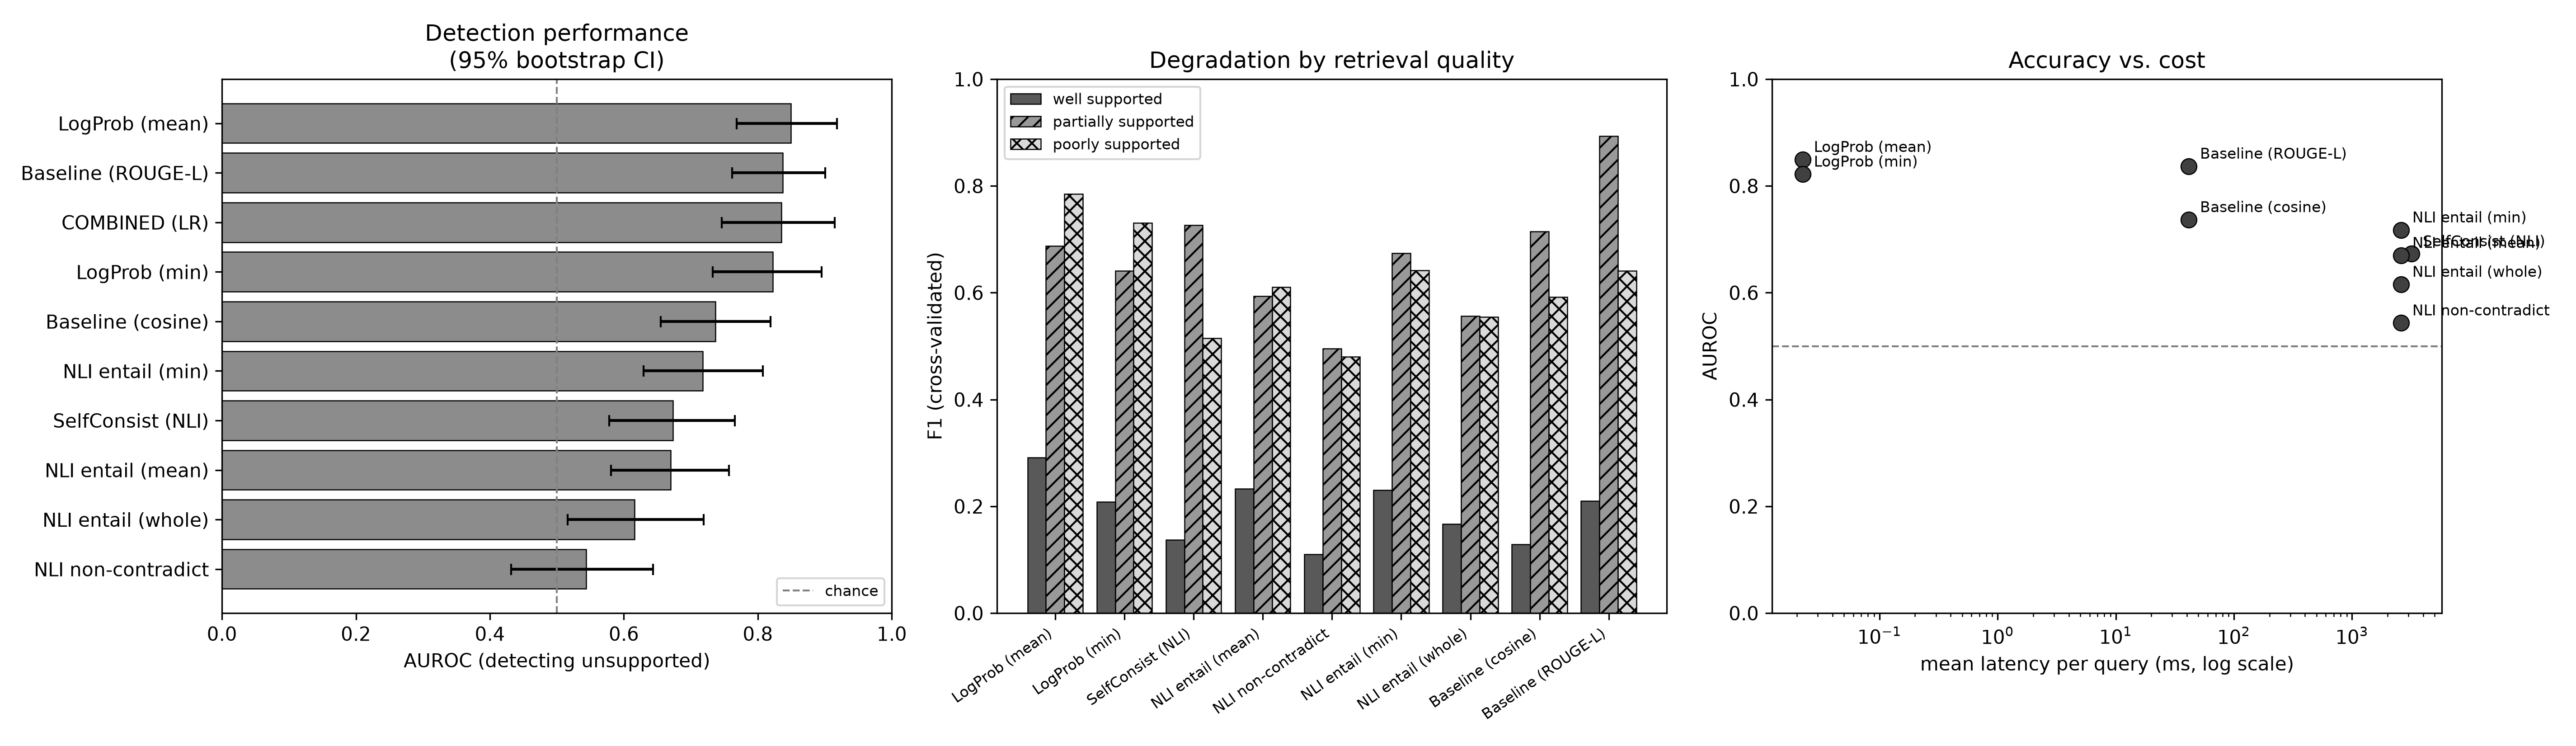
\includegraphics[width=\textwidth]{signals-comparison}
\caption{Left: detection performance with 95\% bootstrap confidence intervals.
Centre: cross-validated $F_1$ by retrieval condition. Right: the accuracy--cost
relationship, with per-query latency on a log scale. The rightmost panel is the
paper's central observation: the points do not trend upward, and the leading
signal sits at the extreme left of the cost axis.}
\label{fig:signals}
\end{figure}

Mean token log-probability is the strongest single signal at AUROC $0.849$, and
it is free, at \SI{0.02}{\milli\second}, essentially the cost of averaging a list
of numbers the generator has already produced. The NLI cross-encoder, at
\SI{2.6}{\second} per query, reaches $0.669$. Self-consistency, the most
expensive signal at \SI{3.2}{\second}, reaches $0.673$.

Because every signal is computed on the same items, the appropriate comparison
is a paired bootstrap of the AUROC \emph{difference} rather than an inspection
of separate intervals, which is both indirect and underpowered. Over 2{,}000
paired resamples, log-probability exceeds NLI-mean by $\Delta = 0.180$
($95\%$ CI $[0.073, 0.279]$, $p < 0.001$) and self-consistency by
$\Delta = 0.177$ ($[0.054, 0.291]$, $p = 0.002$). Its advantage over ROUGE-L is
$\Delta = 0.013$ ($[-0.039, 0.064]$, $p = 0.62$), which is no advantage at all.
We therefore treat the gap to the two expensive signals as established and the
gap to the lexical baseline as absent: the correct reading is that the two
cheapest signals are jointly ahead, not that log-probability alone leads.

The judge arm is the reference point the cheap signals were meant to be
compared against, and it does not perform the role well. Its $F_1$ of $0.589$ is
below the free signal's $0.685$, at roughly \num{200000} times the cost, and its
binary agreement with the human consensus is only $0.693$. The hardened second
prompt performed marginally worse than the first.

Figure~\ref{fig:signals} plots the same data against cost. If detection quality
were purchased with compute, the rightmost panel would trend upward; it does not.
The two cheapest signals occupy the top of the accuracy axis and the far left of
the cost axis simultaneously.

The combined logistic regression ($0.835$) does not improve on its best
component. With four correlated features and 150 items this is unsurprising, but
it is worth stating: on this data there is no combination bonus to be had.

\subsection{Robustness to the binarisation choice}

Collapsing three labels to two involves two decisions, so we repeated the
analysis under all nine combinations of the \emph{partially supported} and
abstention mappings. Log-probability ranges from $0.850$ to $0.979$ across them
and exceeds NLI-mean under every one. The configuration reported above, in which
partial items count as unsupported and abstentions as supported, is the one
under which our headline figure is \emph{lowest}; treating partial items as
supported raises it to $0.923$, and excluding both ambiguous categories raises
it to $0.979$ on the 100 items that remain. We report the least favourable
mapping as the default because it is the most conservative, not because it
flatters the result.

\subsection{Is the signal merely detecting refusals?}

Twenty-eight items are abstentions, which the default mapping counts as
supported, and they concentrate in the poorly-supported condition. This admits
an alternative explanation: if refusals are formulaic and therefore highly
predictable text, log-probability might be separating refusals from
non-refusals rather than grounded answers from ungrounded ones.

It is not. Used to discriminate abstentions from everything else,
log-probability achieves AUROC $0.309$, meaning refusals are if anything
\emph{less} predictable than other answers. Removing abstentions from the
evaluation entirely leaves 122 items and raises log-probability's AUROC from
$0.850$ to $0.907$; NLI-mean rises to $0.777$ and the ordering is unchanged. The
signal is not a refusal detector in disguise, and its performance does not
depend on the abstention convention.

\subsection{Is this just answer length?}

Mean log-probability is length-dependent by construction, so the leading result
requires a check. Answer length alone reaches AUROC $0.724$, and correlates with
mean log-probability at $r = -0.50$. Length is therefore a genuine partial
confound. It does not, however, account for the effect: stratifying into length
terciles, log-probability retains AUROC $0.729$, $0.788$ and $0.861$ within
bands. Unsupported answers are both longer (207 against 162 tokens) and less
confident ($-0.240$ against $-0.160$), which is consistent with a model that
hedges and elaborates when it cannot ground itself.

\subsection{Breakdown by retrieval condition}

\begin{table}[htbp]
\centering
\small
\begin{tabular}{@{}lccc@{}}
\toprule
\textbf{Signal} & \textbf{Well} ($n{=}74$) & \textbf{Partial} ($n{=}26$) &
\textbf{Poor} ($n{=}50$) \\
\midrule
LogProb (mean)      & 0.754 & 0.851 & \textbf{0.852} \\
LogProb (min)       & 0.798 & 0.827 & 0.784 \\
Baseline (ROUGE-L)  & \textbf{0.821} & \textbf{0.979} & 0.770 \\
Baseline (cosine)   & 0.634 & 0.803 & 0.563 \\
NLI entail (min)    & 0.600 & 0.690 & 0.740 \\
NLI entail (mean)   & 0.587 & 0.648 & 0.531 \\
Self-consistency    & 0.592 & 0.785 & 0.674 \\
NLI non-contradict  & 0.570 & 0.488 & 0.431 \\
\bottomrule
\end{tabular}
\caption{AUROC by retrieval condition.}
\label{tab:condition}
\end{table}

Table~\ref{tab:condition} breaks performance down by retrieval condition.
Log-probability is the most stable signal, varying only
between $0.754$ and $0.852$. Most others move considerably more. ROUGE-L reaches
$0.979$ on partially supported items, where the retrieved abstract is correct
but silent on the specific fact asked for; in that setting a model that
fabricates has little context wording to reuse, and lexical overlap separates
the classes almost perfectly. The sample is small ($n = 26$, 12 positive) and the
figure should be read with that in mind.

The non-contradiction signal falls below chance in two of the three conditions.
We had expected it to help, on the reasoning that the neutral/contradiction
distinction maps onto the partially/fully unsupported distinction in our label
scheme. It does not.

Splitting the poorly-supported condition by distractor difficulty shows a
smaller effect than anticipated. Log-probability scores $0.826$ on hard
(same-subfield) negatives against $0.860$ on easy ones; NLI-min moves further,
$0.638$ against $0.806$. With 25 items per cell the intervals are very wide and
we draw no strong conclusion, other than that the cheap signal appears less
sensitive to distractor difficulty than the expensive one.

% ===========================================================================
\section{Discussion}
\label{sec:discussion}

\subsection{Why the cheap signal wins}

The result is easier to accept once one is precise about what mean
log-probability measures. It is not a measure of truth, and not really a measure
of grounding either. It measures how predictable the generated tokens were given
the prompt. When a relevant document sits in the prompt, the most
predictable continuation is one that reuses it. Copying is cheap in
log-probability terms; composing from parametric memory is not.

We should be clear that this is an explanation consistent with the data rather
than one we have tested. Measuring lexical overlap between each answer and its
context, and asking whether that overlap mediates the relationship between
log-probability and the label, would test it directly; we have not done so, and
the strong showing of ROUGE-L, which measures precisely that overlap, is at
least suggestive. If the account is right it also identifies the signal's main
limitation. On this data it works because ungrounded answers are ones the model
had to compose rather than copy. A hallucination that closely mirrors the
wording of the retrieved passage while altering its substance would likely evade
it. Our distractor conditions do not produce many such cases, and a dataset
built to contain them would probably show a different ordering.

The corollary for the NLI signal is less comfortable. It underperforms not
because the model is weak (on controlled pairs it behaves exactly as
documented) but because the unit it is asked to score does not match the unit
LLMs produce. Model answers are long, compound sentences that interleave
supported content with unsupported elaboration, and sentence-level NLI has no
way to report ``three-quarters of this is fine''. The min aggregation collapses
to zero and the mean aggregation dilutes real violations. This is a solved
problem in principle: atomic-fact decomposition \cite{min2023factscore} exists
precisely for it. What our result adds is a cost argument. Once the
decomposition step is included, the NLI approach is not a cheap signal at all,
and it must be compared against a free one that already performs better.

\subsection{Retrieval failure produces refusal, not fabrication}

Our strongest manipulation did not do what it was designed to do. Under poor
support the model refused 40\% of the time, and no well-supported item produced
a refusal at all. Given the wrong document, Qwen2.5-7B usually notices and says
so.

This is partly an artifact of our design. Because the question names the target
paper, the model can compare the requested title against the supplied context
and detect the substitution. The earlier deictic phrasing made that impossible,
but it also made retrieval impossible, so the two are not independent choices.
Any design in which the query is specific enough to retrieve is also specific
enough to make a mismatch detectable.

The consequence is that our positive class is smaller and less adversarial than
intended, and that abstention handling is an analysis flag rather than a
convention. It also suggests that for the wrong-document failure mode
specifically, a well-behaved instruction-tuned model may need less external
checking than assumed, with the interesting residue being the minority of cases
where it fails to notice.

\subsection{The judge is not a reliable ceiling}

We included an LLM judge as the expensive arm of the cost analysis, expecting it
to bound what the cheap signals could achieve. It agreed with the human
consensus only 69.3\% of the time and scored below the free signal.

More instructive is a specific failure. Our judge prompt states explicitly that
an answer correctly declining to answer counts as supported, since it asserts
nothing the context fails to back. Across the 40 refusal-style answers in the
data, the judge applied that rule zero times. To distinguish a property of the
judge from an artifact of our prompt, we re-ran the full set with a second
prompt in which the rubric is unchanged but the abstention rule is lifted out of
the label definition into its own paragraph, given worked examples, and stated as
a prohibition. Compliance moved from 0/40 to 1/40, while verdicts on the 110
non-refusal answers were essentially unchanged. The second prompt did not alter
behaviour broadly; it specifically failed to move the cases its added rule
governs.

We read this as a limitation of LLM-as-judge rather than a prompt-engineering
shortfall: where a rubric and the model's prior disagree, the prior wins, and
further instruction does not recover it. This bears on the framing of the paper.
The usual argument for cheap signals is cost. This suggests a second axis. A
prompted judge can misread a rubric silently and systematically, whereas a
mechanical signal has no rubric to misread: it emits a number, and the mapping
from that number to a decision is the experimenter's, inspectable and adjustable
after the fact. The judge's failure here was invisible without exactly the kind
of audit we happened to perform.

\subsection{Practical recommendation}

For a team deploying RAG on constrained hardware, the ordering in
Table~\ref{tab:overall} suggests a straightforward policy: compute the free
signals first. Mean token log-probability and ROUGE-L recall against the context
together cost under \SI{50}{\milli\second} and, on this data, outperform
everything more expensive.

To make that actionable, an operating point is needed rather than an AUROC. Our
cross-validated threshold flags an answer when its mean token log-probability
falls below $-0.213$, giving precision $0.69$ and recall $0.71$ while flagging
roughly a quarter of answers for review. A deployment prioritising coverage over
reviewer effort can move the threshold to $-0.196$ for $80\%$ recall at
precision $0.56$, flagging $38\%$ of answers. These thresholds are properties of
this generator and this corpus and should be re-fitted rather than transferred;
what transfers is the procedure of fitting them on held-out data, which costs
one pass over a labelled sample and no additional inference. Whether that ordering holds on data containing
context-mimicking hallucinations is an open question, and the honest form of the
recommendation is to measure the free signals on one's own data before
provisioning a judge, rather than assuming, as the literature's framing invites, that
detection quality must be purchased.

% ===========================================================================
\subsection{Limitations}

\paragraph{Sample size.}
With 150 items and 41 positives, confidence intervals are wide and small
differences between signals are not resolvable. We report intervals throughout
and treat overlapping ones as inconclusive. The per-condition and
per-distractor breakdowns rest on 25--74 items each and are correspondingly
weaker.

\paragraph{Clustered items.}
The 150 questions derive from only 50 abstracts, three per paper, so items
sharing a source are not independent. The effective sample size lies somewhere
between 50 and 150, which is a further reason to prefer the bootstrap intervals
over point estimates.

\paragraph{A single generator.}
All signals are measured against one 7B model at one quantisation level. Signal
behaviour plausibly depends on scale and calibration, and log-probability in
particular is a property of the specific decoder. We do not vary this.

\paragraph{The log-probability result may not transfer.}
As argued in Section~\ref{sec:discussion}, the signal appears to work here
because ungrounded answers were composed rather than copied. A dataset built to
contain fluent, context-mimicking fabrications would test this directly, and we
would not expect the ordering to survive unchanged.

\paragraph{Claim granularity.}
We decompose answers into sentences, but LLM sentences are compound and NLI
marks a whole sentence non-entailed if any clause is unsupported. This is why
the strict aggregation collapses and why even the mean variant is probably
pessimistic on correct answers. Atomic-fact decomposition would give a cleaner
measurement; we did not implement it.

\paragraph{The poorly-supported condition is milder than intended.}
Because the model can detect the paper substitution, that condition yields a
high rate of appropriate refusal rather than fabrication. Results should not be
read as characterising signal behaviour under \emph{undetectable} retrieval
failure, which is a harder and arguably more realistic setting.

\paragraph{A partly circular criterion.}
Our annotation criterion asks whether the context supports the answer's claims,
which is close to what an NLI model computes. Had the NLI signal performed well,
that closeness would warrant caution. It performed poorly, so the concern does
not arise in this instance, but it would apply to any future work that improves
the decomposition.

\paragraph{Hardware.}
Latency was measured on a single power-limited consumer GPU running at roughly a
fifth of its rated throughput. Relative ordering across signals is unaffected,
since all were timed identically, but absolute figures are upper bounds.

% ===========================================================================
\section{Conclusion}

We compared three inference-time hallucination-detection signals on a
150-item RAG benchmark under a strict hardware constraint, measuring cost
alongside accuracy. On our data the ordering runs opposite to the one the
literature's framing implies. Mean token log-probability, which is free and requires
nothing beyond numbers the generator already computes, led on AUROC at $0.849$
and beat both expensive signals by a paired margin of roughly $0.18$
($p \le 0.002$), while an NLI cross-encoder reached
$0.669$ at \SI{2.6}{\second} per query and a 7B LLM judge scored a lower $F_1$
than the free signal at \SI{5.0}{\second}, agreeing with human annotators only
69.3\% of the time. It was not, however, distinguishable from a
\SI{41}{\milli\second} lexical baseline, so the finding is better stated as
cheap signals outperforming expensive ones than as any single signal winning.

We do not claim log-probability is a better hallucination detector in general.
The mechanism we propose, that it separates copied text from composed
text, predicts that it should fail on fabrications which mimic the retrieved
context closely, and our data contains few of those. What we do claim is
narrower and, we think, more useful: that the assumption of a monotonic
relationship between detector cost and detector quality does not survive
measurement, at least here, and that a team building a RAG system should
measure the free signals on their own data before provisioning anything larger.

Two further findings emerged that we did not set out to test. A well-behaved
instruction-tuned model refuses rather than fabricates in a substantial fraction
of wrong-document cases, which shifts where detection effort is best spent. And
an LLM judge violated an explicit, repeatedly emphasised instruction in its own
rubric on essentially every applicable case, a reminder that a judge baseline
is an object of study rather than a source of truth.

Future work should test the log-probability result against adversarially
context-mimicking hallucinations, implement atomic-fact decomposition so that
the NLI comparison is a fair one, and repeat the comparison across generator
scales, since a signal read off a decoder's own probabilities is unlikely to
behave identically across model sizes.

% ===========================================================================
\section*{Declarations}

\paragraph{Funding.}
No funding was received for this work.

\paragraph{Conflicts of interest.}
The authors declare no conflicts of interest.

\paragraph{Data availability.}
The corpus, the 150 generated answers with their token log-probabilities and
sampled generations, the per-annotator and consensus label files, all signal
scores, and the full analysis pipeline are available from the corresponding
author on request and will be released publicly on acceptance. Because arXiv
relevance ranking drifts over time, the corpus file rather than the search query
is the artifact of record, and it is included.

\paragraph{Use of generative AI.}
A large language model (Anthropic Claude, Opus 5) was used substantially in this
work, and we set out its role in full. It wrote the experimental pipeline: the
retrieval index, the generation harness, the signal computation, and the
evaluation and plotting scripts. It performed the statistical analyses reported
in Section~\ref{sec:results}, including the bootstrap intervals, the paired
comparisons, and the length-stratified check. It produced drafts of the
manuscript text, which the authors revised. It also proposed the initial
reference list.

Three things were not done by the tool. The authors designed the study and made
every experimental decision, including the corpus construction, the retrieval
conditions, and the choice of signals. The authors produced all annotation
personally; no label in the ground-truth set originated from a generative model,
and the human labels are what every result in this paper is measured against.
And the authors verified every reference against the publisher record rather
than accepting the tool's output: page numbers and author lists were corrected
where the initial output was incomplete or wrong.

The authors take responsibility for the entire content of the manuscript,
including any error that survived this process.

% ===========================================================================
\bibliographystyle{apacite}
\bibliography{references}

\end{document}
